\chapter{Introduction}

\section{Objecte}


Resultat final que es vol aconseguir. En aquest cas, l’objecte d’aquesta plantilla és donar les pautes d’estructura i contingut de la Memòria del TFE. 

El cos tant d’aquest document “Memòria” com dels altres documents integrants del TFE  (Pressupost, Annexos i Plec de condicions) serà amb lletra Times New Roman o Arial d’una mida d’11 punts, marge lateral esquerra de 3 cm, dret de 2,5, superior i inferior de 2,5 i espaiat senzill.

L’alumne/a ha de revisar l’ortografia i gramàtica de tots els documents del TFE; ha d’utilitzar les unitats del Sistema Internacional; ha d’utilitzar un nombre coherent de decimals; i ha d’identificar els eixos dels gràfics inclosos al llarg del text.

Es recomana que la memòria no superi una extensió màxima de 60-70 pàgines. 
Tant les taules com figures han d’estar enumerades i tenir un títol. Si s’han obtingut d’algun altre document consultat, s’haurà de dir la font d’on s’ha tret \cite{eseiaat}.


\begin{figure}[H]
    \centering
    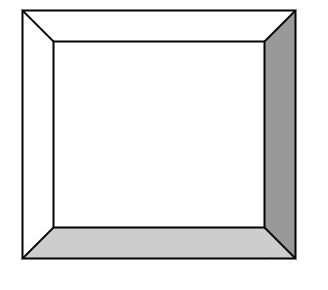
\includegraphics[width=0.3
\linewidth]{Figures/IMATGE_EXEMPLE.jpg}
    \caption{Imatge d'exemple}
    \label{fig:Imatge d'exemple}
\end{figure}


\begin{table}[H]

  \centering
   \caption{Risks assessment} 
   
  \begin{tabular}{|c|c|c|c|}
    \hline
    \textbf{1} & \textbf{X2} & \textbf{X} & \textbf{X} \\ \hline
    ... & ... & ... & ...\\ \hline
    ... & ... & ... & ...\\ \hline
    ... & ... & ... & ...\\ \hline
    ... & ... & ... & ...\\ \hline
    
  \end{tabular}
  \label{tasks}
 
\end{table}


\section{Abast}

Paquets de treball i lliurables necessaris per arribar a la solució.

\section{Requeriments}

O especificacions bàsiques. Restriccions sobre la solució final.

\section{Justificació}

Plantejament de la necessitat del treball des d’una visió global i aproximant-lo a una visió més específica. Serveix per centrar i contextualitzar el treball.


\subsection{Subsection}

\subsubsection{superseccion}

\begin{minted}[label=\texttt{divisiones.py}]{python3}
	"""
	Biblioteca con definiciones importantes para la división de números.
	Se incluyen las funciones divideSiDivisible() y cocienteModulo().
	"""
	
	def divideSiDivisible(nume, deno):
	"""
	Si nume es divisible por deno, devuelve la división
	entera. Si no lo es, devuelve None.
	"""
	
	if not nume % deno:
	return nume // deno
	
	
	def cocienteModulo(nume, deno):
	"""
	Devuelve el conciente entero y el resto de
	la divisi
	ón entera (mod) de dos números.
	"""
	
	return nume // deno, nume % deno
	
\end{minted}


\inputminted[label={src/divisions.py},firstline=6,lastline=13]{python}{src/divisions.py}

